% !TeX encoding = UTF-8
% !TeX program = pdflatex
% !BIB program = bibtex

%%% Um einen Artikel auf deutsch zu schreiben, genügt es die Klasse ohne
%%% Parameter zu laden.
\documentclass[english]{lni}
%%% To write an article in English, please use the option ``english'' in order
%%% to get the correct hyphenation patterns and terms.
%%% \documentclass[english]{class}
%%

\usepackage{booktabs}
\usepackage{pgfplots}

\pgfplotsset{width=12.5cm, height=4cm}

\begin{document}
%%% Mehrere Autoren werden durch \and voneinander getrennt.
%%% Die Fußnote enthält die Adresse sowie eine E-Mail-Adresse.
%%% Das optionale Argument (sofern angegeben) wird für die Kopfzeile verwendet.
\title[From Facts to Rules using Relational Databases]{From Facts to Rules using Relational Databases}
%%% \subtitle{From Facts to Rules using Relational Databases} % if needed
\author[Tim Gutberlet \and Janik Sauerbier]
{Tim Gutberlet\footnote{University of Mannheim, \email{tgutberl@mail.uni-mannheim.de}} \and
Janik Sauerbier\footnote{University of Mannheim, \email{jsauerbi@mail.uni-mannheim.de}}}
\startpage{1} % Beginn der Seitenzählung für diesen Beitrag / Start page
\editor{K.-U. Sattler et al.} % Names of Editors
\booktitle{Datenbanksysteme für Business, Technologie und Web (BTW 2023)} % Name of book title
\yearofpublication{2023}
%%%\lnidoi{18.18420/provided-by-editor-02} % if known
\maketitle

\begin{abstract}
In this paper, we focus on the problem of finding all rules that imply a certain target fact given a knowledge graph and a set of previously learned rules over the knowledge graph. We specifically analyze how relational database technology performs in solving this problem using indexing, filtering and pre-processing methods. Our research might help to advance approaches for link prediction and can be used to efficiently explain the dynamics of rules given large amounts of target facts or large knowledge graphs.

Test
\end{abstract}
\begin{keywords}
Knowledge graph completion \and Link prediction \and Knowledge representation and reasoning \and Relational databases.
\end{keywords}
%%% Beginn des Artikeltexts
\section{Introduction}
Knowledge graphs (KGs) are used in different fields from biomedical applications \cite{OpenBioLink} over applications in the context of social networks \cite{SocialNetworks} to semantic search applications\cite{SemanticSearch}. We want to contribute by analyzing how to effectively check which rules of a KG imply certain target facts using relational database technology. For the rule learning, we use AnyBURL, a fast bottom up rule learner for KGs.\cite{AnyBURL19}

Our research might be used as a primitive for the link prediction problem. Prior research indicates that rule-based approaches and embedding models can be used in combination to improve inference quality.\cite{RuleEmbeddingCombination1}\cite{RuleEmbeddingCombination2} There is a significant need for a time-efficient solution that is used to check which rules implicate certain facts. Beyond potentially facilitating faster link prediction, our findings can already be helpful to explain the dynamics of rules given large amounts of potential facts for KGs. It might also particularly help in case of large knowledge graphs and memory constraints. 

To achieve those goals, we ran several experiments aimed to illustrate how different database setups impact the performance in terms of execution time using filtering, indexing and pre-processing methods. Beyond that, we also performed a quantile performance analysis on the queries and rules.

\section{Preliminaries} 
A knowledge graph is a set of triples (subject, relation, object) that describe a directed graph. The edges are represented by the relations going from subject to object. The nodes are the set of entities which appear as subjects and objects of the triples. The individual triples are also called facts. KGs can be used to describe various domains and to identify rules and patterns in those domains. For our purposes, we are concerned about first-order logic Horn rules. These rules consist of a head and a body, where the head consists of one triple and the body consists of one or more triples. The subjects and objects of the triples can either be specific entities or variables. Here are two example rules. We use the notation relation(subject, object) for the triples and capitalize the variables.

\begin{equation}
citizenOf(X, germany) \leftarrow bornIn(X, mannheim) 
\end{equation}
\begin{equation}
livesIn(X, germany) \leftarrow marriedTo(X, A_1), bornIn(A_1, germany)
\end{equation}

The grounding of a rule is a set of triples of the KG that fulfil the rule, with matching entities for all variables. The triple set \textit{\{livesIn(tom, germany), marriedTo(tom, bob), bornIn(bob, germany)\}} would be a grounding for the second rule.

\section{Problem Statement}
The problem we are trying to solve is identifying rules that imply certain target facts which are not part of the KG based on the KG and a previously learned set of rules. This means we are looking for a grounding of the rule with the target triple matching the head of the rule and a subset of triples from the KG matching the body of the rule. To illustrate the problem, think of the following example.

\begin{itemize}
  \item \textbf{Knowledge Graph:}
  \item[] \(\{…, marriedTo(anna, peter), bornIn(peter, germany), …\}\)
  \item \textbf{Target Fact:} \(livesIn(anna, germany)\)
  \item \textbf{Learned Rules:}
  \begin{enumerate}
      \item \(citizenOf(X, germany) \leftarrow bornIn(X, mannheim)\)
      \item \(livesIn(X, germany) \leftarrow marriedTo(X, A_1), bornIn(A_1, germany)\)
  \end{enumerate}
\end{itemize}

In our example we can start off with excluding rule one from further investigation as the target fact needs to match the head of the rule. Rule two has a matching head with \(X = anna\). To investigate whether rule two actually implies the target fact, we need to find matching facts for the rule body from the KG. The KG contains the facts \(marriedTo(anna, peter)\) and \(bornIn(peter, germany)\). Together with the target fact, this results in a grounding for the second rule with \(X = anna\) and \(A_1 = peter\). Therefore, rule two is part of the solution.

\section{Implementation}

Our solution was implemented using the open-source object-relational database system PostgreSQL. The basic idea behind our implementation is creating SQL queries for each target fact. The given KG will be stored in one table of the relational database (columns: “sub” for subjects, “pre” for relations and “obj” for objects). The SQL statement consists of \textit{UNION ALL} operations over all sub-queries for the individual rules. The rules are saved in a list and in a loop over all rules, the sub-queries for rules with matching heads are created. To improve this basic idea, we employed several optimizations listed below. This would be the query for the example given in the problem statement:

\textit{(\textbf{SELECT} rule\_1 \textbf{FROM} kg\_table t0,  kg\_table t1 \textbf{WHERE} k0.sub = anna \textbf{AND} k0.obj = k1.sub \textbf{AND} k1.obj = germany \textbf{LIMIT} 1)  \textbf{UNION ALL} (...)}


\subsection{Hash Maps for Rule Pre-filtering} 
To speed up the pre-filtering of the rules, we sorted the given set of rules into a hash map with five keys based on the rule head type. Three of the head types have fixed entities, either as subject and/or as object [e.g., \textit{r1(e1, X)}, \textit{r1(X, e1)} or \textit{r1(e1, e2)}]. Two of the head types have a variable as subject and as object, either the same variable or different variables [e.g., \textit{r1(X, X)}, \textit{r1(X, Y)}]. Within the respective categories, the rules are again sorted into hash maps based on the relation and the fixed entities. This allows for initial filtering of the rules in O(1).

\subsection{Tables for each Relation}
We created an alternative approach to having one big table for all facts of the KG. This approach uses one table for each relation in the KG therefore decreasing the individual table size. They only contain two columns for the subject and the object. This solution improved the overall performance by reducing the size of the B-trees of the indexes.

\subsection{Indexing}
To speed up the joining of the tables, we duplicated the knowledge graph tables and employed a unique clustered index, once with (subject, object) as key and once with (object, subject) as key. Within the SQL statement, the tables with the order (subject, object) are used in case of a fixed subject and the tables with the order (object, subject) are used in the case of a fixed object or no fixed subject and object. This ensures that an index is used as often as possible. The index speeds up the search and enables the direct access to the table contents through the B-trees.

\subsection{Pre-processing of expensive Rules}
As we will illustrate in our experiments, certain rules are way more expensive than others. To address that, we integrated a simple pre-processing method. We gather an independent set of n facts and used them as target facts. The queries were amended with the \textit{EXPLAIN ANALYZE} command to get the execution time for the individual rule sub-queries. Afterwards, we ranked all rules by the sum of the execution time over all queries. The top x\% of rules were then pre-processed, by calculating all potential rule heads which could form a grounding together with a set of triples from the KG as rule body. We excluded rules with one body triple, as pre-processing didn’t improve the performance. We also excluded rules with more than two body triples, as those rules incur a pre-processing time two orders of magnitude higher than rules with two body triples, while they only make up a small fraction of the most expensive and frequent rules.


\section{Experiments}
The goal of our experiments was to benchmark the performance of our solution and to measure the effects of different optimizations. We also analyzed the execution time for individual queries and rules. Beyond that, we tested our solution on different datasets and rulesets. Our solution is written in Java using the PostgreSQL JDBC driver. The source code and datasets, used in the experiments, can be found at https://github.com/timgutberlet/From-Facts-to-Rules-using-Relational-Databases. We conducted all experiments on a Fujitsu Esprimo P957 (construction year 2017) with 32 GB RAM, 512 GB SSD, an Intel i7-7700 @ 3.6 GHz CPU and Ubuntu 22.04.1 LTS as an operating system.

\subsection{Ablation Study - Optimizations} 

\begin{table}
\centering
\begin{tabular}{lll}
\toprule
Experiment & Avg. Execution Time \\
\midrule
All optimizations enabled & 10 ms\\
\midrule
Hash Maps for Rule Pre-filtering disabled & XX ms\\
Tables for each relation disabled & 140 ms\\
Indexing disabled & 1680 ms\\
Pre-processing of expensive rules disabled & 11 ms\\

\bottomrule
\end{tabular}
\caption{Ablation Study of Optimizations using YAGO3-10}
\label{tab:ablation}
\end{table}

For these experiments, we used YAGO3-10 as the benchmark dataset.\cite{YAGO3} The dataset consists of a training set (1079040 triples), test set and validation set (5000 triples each). We used AnyBURL to learn rules for 50 seconds, only generating rules that do not have empty bodies (107301 Rules). We used the training set as the KG and the validation set as the target triples. For the \textit{Pre-processing of expensive Rules} optimization, we use the test set (n = 5000) to create the rule ranking and pre-process the top 1\% rules. The results in \Cref{tab:ablation} are based on executing all 5000 queries.

The \textit{Tables for each Relation} optimization specifically reduced the execution time for long rules. For rules with one body triple, the execution time was reduced by 12\%, for two body triples by 25\% and for three body triples by 74\%. This is caused by the increased use of the indexes during execution.

\subsection{Quantile Performance Analysis} 

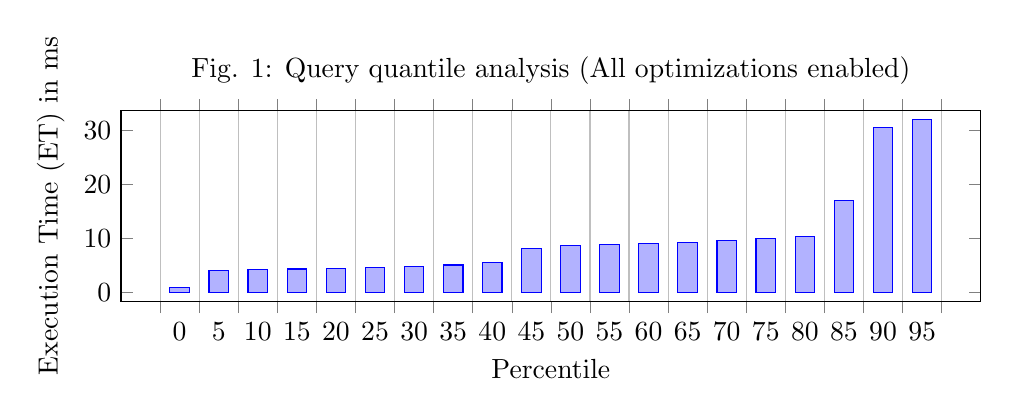
\begin{tikzpicture}
\begin{axis}[
        title={Fig. 1: Query quantile analysis (All optimizations enabled)},
	x tick label style={
		/pgf/number format/1000 sep=},
	ylabel=Execution Time (ET) in ms,
        xlabel=Percentile,
	enlargelimits=0.05,
	legend style={at={(0.5,-0.1)},
	anchor=north,legend columns=-1},
	ybar interval=0.5,
]
\addplot 
	coordinates {(0, 0.984156) (5, 4.113395)
            (10, 4.242852) (15, 4.38007)
            (20, 4.5406935) (25, 4.6855745)
            (30, 4.860181) (35, 5.1234675)
            (40, 5.626696) (45, 8.143013)
            (50, 8.648211) (55, 8.905306)
            (60, 9.140784) (65, 9.355278)
            (70, 9.636537) (75, 9.959422)
            (80, 10.475147) (85, 17.016464)
            (90, 30.580482) (95, 32.047903) 
            (100, 0)};
\end{axis}
\label{Test}
\end{tikzpicture}

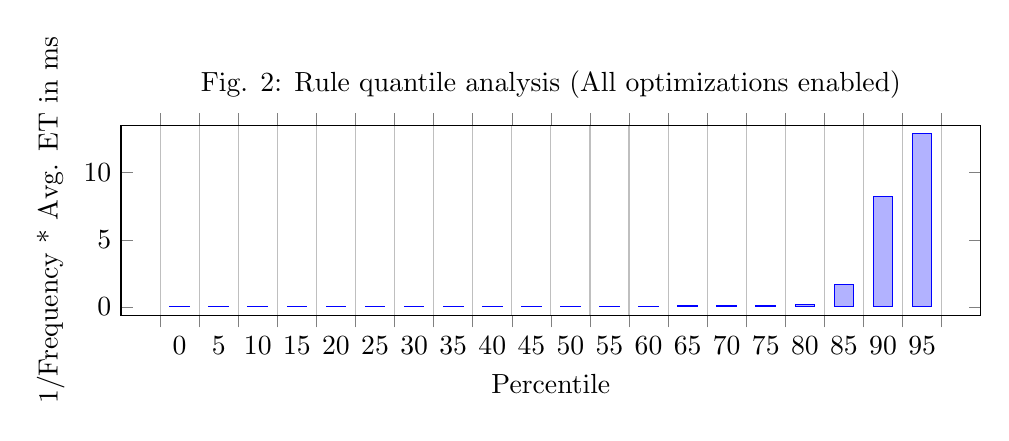
\begin{tikzpicture}
\begin{axis}[
        title={Fig. 2: Rule quantile analysis (All optimizations enabled)},
	x tick label style={
		/pgf/number format/1000 sep=},
	ylabel=1/Frequency * Avg. ET in ms,
        xlabel=Percentile,
	enlargelimits=0.05,
	legend style={at={(0.5,-0.1)},
	anchor=north,legend columns=-1},
	ybar interval=0.5,
]
\addplot 
	coordinates {(0, 0.021) (5, 0.025)
            (10, 0.026) (15, 0.027)
            (20, 0.027) (25, 0.028)
            (30, 0.030) (35, 0.031)
            (40, 0.032) (45, 0.036)
            (50, 0.042) (55, 0.052)
            (60, 0.057) (65, 0.064)
            (70, 0.08) (75, 0.1)
            (80, 0.152) (85, 1.64)
            (90, 8.26) (95, 12.90) 
            (100, 0) };
\end{axis}
\label{Test}
\end{tikzpicture}

The analysis indicates that only few rules and few queries incur a major share of the cost. The \textit{Pre-processing of expensive Rules} optimization helped to reduce the cost for very expensive rules. The execution time for a specific rule is influenced by the length of the rule, as well as the target triple and the structure of the knowledge graph.

\subsection{Further Datasets and Rulesets}

\begin{table}
\centering
\begin{tabular}{llll}
\toprule
 & AnyBURL - 10s & AnyBURL - 50s & AnyBURL - 100s\\
\midrule
YAGO3-10 & XX ms & 10 ms & XX ms\\
WN18RR & XX ms & XX ms & XX ms\\
FB15k-237 & XX ms & XX ms & XX ms\\
\bottomrule
\end{tabular}
\caption{Average Execution Time for different Datasets and Rulesets}
\label{tab:further-datasets}
\end{table}

Our solution works for different datasets and rulesets learned by AnyBURL in the given time. The solution is particularly well suited for datasets with many relations, like the Freebase dataset, as it allows for small B-trees of the indexes.



%However, to show the relevance of our approach, we also tested the performance of our optimisation strategies, without limiting the rule types in any sense.

%Conclusions / Assumptions:
%Yago3 - 10 has relatively low amount of 37 different relations. Working with datasets with a higher count of relations could possibly improve the approach of using materialized views for every relation, as the knowledgegraph would be split even more fine-grained. 


\section{Conclusions}

%
% the environments 'definition', 'lemma', 'proposition', 'corollary',
% 'remark', and 'example' are defined in the LLNCS documentclass as well.
%

We demonstrated an effective solution for finding all rules that imply a certain target fact given a knowledge graph and a set of previously learned rules. Our experiments specifically demonstrated the effect of filtering, indexing and pre-processing methods. Potential next steps include a further analysis of our solution on various datasets, a comparison of different database technologies (particularly triplestores), exploring the use of multithreading and creating a dedicated solution only using the main memory.

\textbf{Acknowledgement.} This paper would not have been possible without the exceptional support of our supervisor, Prof. Dr. Rainer Gemulla.

%%% Angabe der .bib-Datei (ohne Endung) / State .bib file (for BibTeX usage)
\bibliography{references} %\printbibliography if you use biblatex/Biber
\end{document}
